\chapter{Metodologia proposta}\label{cap:metodologia}

Existem diversas oportunidades para desenvolvimento de novos algoritmos de otimização e busca local, utilizando recursos de programação paralela.
Neste trabalho é proposta uma implementação em dataflow do DVND e apresentado GDVND conforme se verá a seguir.

\section{RVND}

O RVND, conforme descrito na Seção~\ref{sec:rvndClassico}, pode ser implementado num grafo dataflow conforme a Figura~\ref{fig:rvndGraph}, onde o nó inicial (\textit{ini}) envia a solução inicial para o primeiro operador de vizinhança (\textit{Swap}), cada nó operador de vizinhança explora todos os movimentos e escolhe o melhor, se este melhora a solução atual então a solução melhorada é enviada para o primeiro né operador (\textit{oper0}) caso contrário a solução é enviada para o próximo nó de enumeração de vizinhança.

\begin{figure}[htbp]
    \centerline{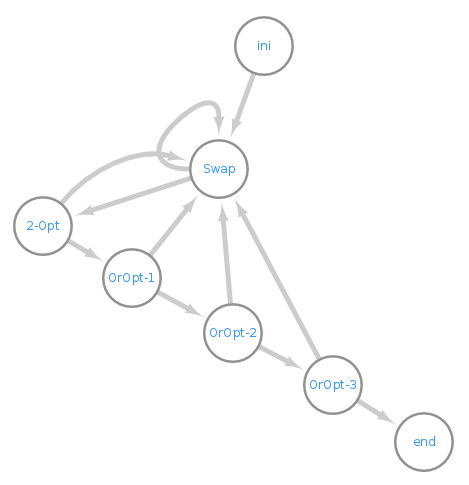
\includegraphics[scale=0.5]{figuras/rvnd/RVND_dataflow_nomes.png}}
    \caption{Arquitetura simplificada do dataflow para o RVND com as vizinhanças utilizadas.}
    \label{fig:rvndGraph}
\end{figure}

A implementação do nó operador (\textit{Swap, 2-Opt, OrOpt-1, OrOpt-2, OrOpt-3}) é tão simples quanto o Algoritmo~\ref{alg:rvndOper} e cada estratégia de vizinhança é atrelada a um nó operador, sendo que a ordem desses é variada para cada execução do método para caracterizar o RVND, a decisão de para qual nó enviar o resultado é tomada pela configuração do dataflow.
Quando a solução atinge o nó final (\textit{end}) esta é salva e o processo termina.

\begin{algorithm}[htpb]
\caption{Nó de vizinhança do RVND}
\label{alg:rvndOper}
\begin{algorithmic}[1]
    \Function{RVND\_Oper}{Solução: $s$}
        \Let{$s'$}{melhor solução de $N^k(s)$}
        \Let{$improvFlag$}{$f(s') < f(s)$}
        \Return{$(s', improvFlag)$}
    \EndFunction
\end{algorithmic}
\end{algorithm}

Pode ser visto destacado na Figura~\ref{fig:rvndGraphDestacado} uma vizinhança com suas ligações ao grafo dataflow, uma de entrada de dados e duas outras de saída que são para o caso de haver ou não uma melhoria no valor da solução.
Para acoplar uma nova vizinhança ao algoritmo basta que seja inserido um novo nó de enumeração com sua entrada de dados vindo do nó anterior e duas saídas de dados, uma retornando para a primeira vizinhança e outra para a vizinhança seguinte, conforme destacado na mesma figura.

\begin{figure}[htbp]
    \centerline{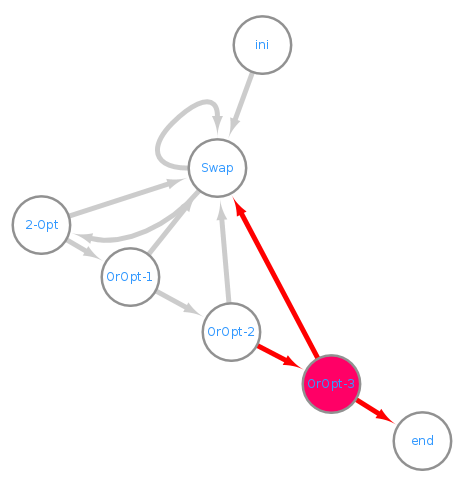
\includegraphics[scale=0.5]{figuras/rvnd/RVND_dataflow_nomesDestacado.png}}
    \caption{Uma vizinhança e suas ligações ao grafo dataflow no RVND.}
    \label{fig:rvndGraphDestacado}
\end{figure}

\subsection{Passo iterativo}

Utilizando o termo convencionado na seção~\ref{subsec:passoIterativo}, cada passo iterativo do RVND retorna a melhor solução encontrada para a vizinhança atual.
Assim sendo $N^k$ a vizinhança atual temos o passo iterativo para o RVND expresso na Equação~\ref{eq:rvndPassoIterativo}.
\begin{equation} \label{eq:rvndPassoIterativo}
    \rho^{RVND}(s) = s' \in N^k \quad \textrm{sendo} \quad f(s') < f(s''), \forall s'' \in N^k(s) \land s'' \ne s
\end{equation}
Fazendo uso da notação de movimentos temos podemos escrever \ref{eq:rvndPassoIterativo} como a Equação~\ref{eq:rvndPassoIterativoMovimento}.
\begin{equation} \label{eq:rvndPassoIterativoMovimento}
    \rho^{RVND}(s) = m \circ s \quad \textrm{com} \quad m \in M^k \land \widehat{m} < \widehat{m_i} \mid \forall m_i \in M^k
\end{equation}

\section{DVND}\label{subsec:dvnd}

Foi descrito na Seção~\ref{sec:dvndClassico} o algoritmo do DVND, contudo um modelo dataflow para o DVND pode ser visto na Figura\ref{fig:dvndGraph}, o método usa $P + 1$ nós iniciais (\textit{ini0}, \textit{ini1}, \dots \textit{iniP}) que alimentam os nós operadores (\textit{Swap, 2-Opt, OrOpt-1, OrOpt-2, OrOpt-3}) e o nó gerente (\textit{man}) com a solução inicial para a busca local.

\begin{figure}[htbp]
    \centerline{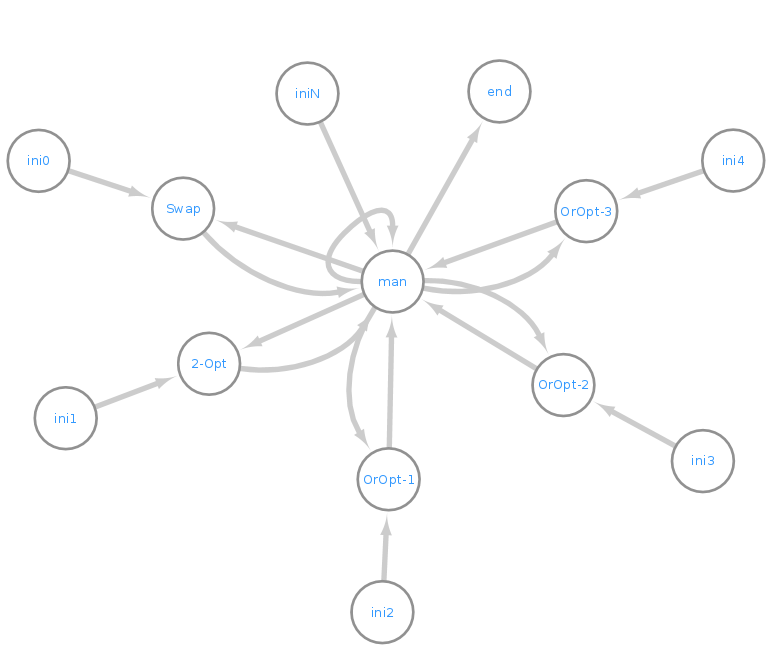
\includegraphics[scale=0.6]{figuras/dvnd/DVND_dataflow_nomes.png}}
    \caption{Arquitetura simplificada do dataflow para o DVND com as vizinhanças utilizadas.}
    \label{fig:dvndGraph}
\end{figure}

Cada nó operador utiliza uma estratégia de vizinhança diferente, quando termina de enumerar as soluções este retorna a melhor para o nó gerente que mantém a melhor solução encontrada até o momento.
Então o nó gerente identifica a melhor solução conhecida e a envia de volta para o dataflow (como no Algoritmo.~\ref{alg:dvndMan}) que encaminha a solução para todos os nós operadores parados, o processo se repete até que nenhum nó operador encontre uma solução melhor.
Então a melhor solução encontrada é enviada para o nó final (\textit{end}) que salva o resultado da busca local.

\begin{algorithm}[htpb]
\caption{Nó \textit{man} do DVND}
\label{alg:dvndMan}
\begin{algorithmic}[1]
    \Function{DVND\_Man}{Solução: s, Histórico: H}
        \Let{$H$}{$H \cup \{s\}$}
        \Return{$bestSolution(H)$}
    \EndFunction
\end{algorithmic}
\end{algorithm}

O critério de parada é alcançado quando nenhum nó operador consegue melhorar a solução atual significando que está corresponde a ótimo local para todas as vizinhanças usadas no processo.
Este é, de certa forma, o mesmo critério utilizado por ambos RVND e DVND, contudo o caminho percorrido pelos diferentes processos pode levar a a ótimos locais diferentes. Tanto para o RVND quanto DVND as estratégias de vizinhança são atribuídas aos nós \textit{oper} e os métodos não definem o comportamento interno destes nós facilitando sua alteração ou mesmo a adição de uma nova vizinhança.

\begin{figure}[htbp]
    \centerline{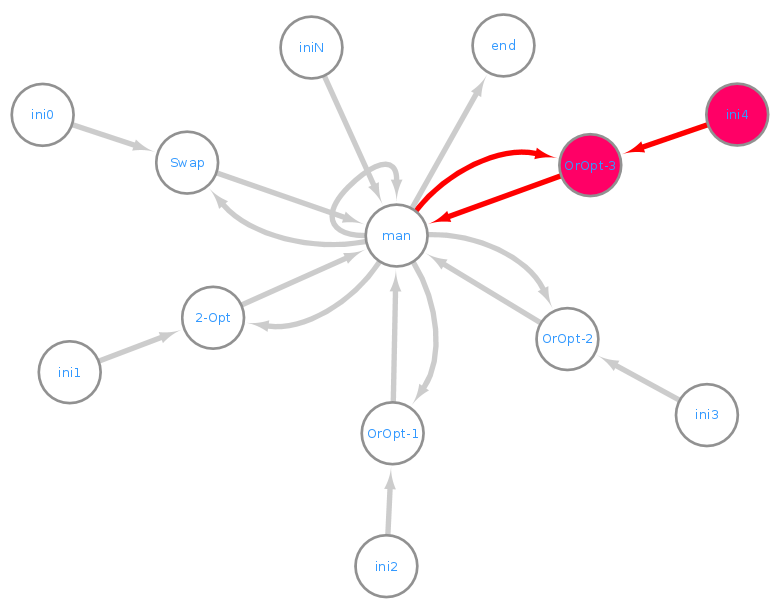
\includegraphics[scale=0.6]{figuras/dvnd/DVND_dataflow_nomesDestacado.png}}
    \caption{Uma vizinhança e suas ligações ao grafo dataflow no DVND.}
    \label{fig:dvndGraphDestacado}
\end{figure}

Como dito anteriormente, qualquer vizinhança pode ser facilmente acoplada ao procedimento apenas adicionando um novo nó operador \textit{oper} ao grafo dataflow, conforme destacado na Figura~\ref{fig:dvndGraphDestacado}, o que é uma grande característica do método, e como os nós são independentes é possível fazê-lo sem impactar nos outros nós.
Inicialmente pode parecer que muitos nós operadores podem sobrecarregar o nó gerente, mas é importante notar que o tempo computacional gasto pelos nós operadores é geralmente muito mais caro (exploração das vizinhanças é o processo mais caro de uma meta-heurística), desta forma não será um grande problema mesmo quando os nós operadores responderem em tempos curtos.

No trabalho apresentado em~\cite{df-dvnd2018} o modelo dataflow usado possuía apenas uma porta de saída então a mensagem seria enviada para todos os nós a ele vinculados, numa melhoria a esta implementação foi implementado e sugerido um aperfeiçoamento ao Sucuri para comportar portas de saída diferentes para destinos diferentes.
No modelo proposto (veja Figura~\ref{fig:dvndGraph}), o nó gerente é ligado a todos os nós operadores o que causaria uma inundação (\emph{flooding}) na rede, desta forma possuir mais de uma porta de saída permite evitar que um nó processe indevidamente uma solução ou que receba uma mensagem com uma indicação de que não deve ser processada o que causaria uma troca de mensagens desnecessária, problema esse que se intensifica ao rodar o processamento em rede.
Um problema que permanece é o escalonador centralizado, o que significa que num processamento em rede cada mensagem precisa ser enviada de volta para o computador rodando o nó gerente para só então ser enviada para o seu nó de destino, incluindo nisso as mensagens de \emph{feedback} explicadas no Sub-seção~\ref{text:flipFlop}.
Contudo a disponibilização de um escalonador distribuído demandaria um novo projeto para a o dataflow do DVND (Figura~\ref{fig:dvndGraph}) de forma a fazer melhor uso deste recurso.
Apesar das limitações atuais deste projeto em desenvolvimento, o Sucuri já provê um ambiente que pode ser facilmente escalado de uma máquina para um experimento em rede completamente distribuído.

\subsection{Passo iterativo}

Utilizando o termo convencionado na seção~\ref{subsec:passoIterativo}, cada passo iterativo do DVND retorna a melhor solução encontrada para todas as vizinhanças.
Dessa forma, sendo $N$ a união de todas as vizinhanças, o passo iterativo do DVND pode ser dado pela Equação~\ref{eq:dvndPassoIterativo}.
\begin{equation} \label{eq:dvndPassoIterativo}
\rho^{DVND}(s) = s' \in N \quad \textrm{com} \quad f(s') < f(s''), \forall s'' \in N(s) \land s'' \ne s
\end{equation}
Fazendo uso da notação de movimentos podemos escrever \ref{eq:dvndPassoIterativo} como a Equação~\ref{eq:dvndPassoIterativoMovimento}.
\begin{equation} \label{eq:dvndPassoIterativoMovimento}
\rho^{DVND}(s) = m \circ s\quad \textrm{com} \quad m \in \mathcal{M} \land \widehat{m} < \widehat{m_i} \mid \forall m_i \in \mathcal{M}
\end{equation}

Pelo passo iterativo do RVND $\rho^{RVND}$ (\ref{eq:rvndPassoIterativoMovimento}) e do DVND $\rho^{DVND}$ (\ref{eq:dvndPassoIterativoMovimento}) podemos concluir que $\rho^{DVND}(s) \le \rho^{RVND}(s)$, contudo isso não é suficiente para afirmar que o DVND encontre necessariamente melhores resultados.% pois o DVND pode acabar convergindo muito cedo para um mínimo local.

\subsection{Nó de flip flop}\label{subsec:flipFlop}

É esperado um comportamento sem estado para os nós num grafo de uma arquitetura dataflow contudo no modelo do DVND proposto (veja Figura~\ref{fig:dvndGraph}) o nó gerente precisa manter o histórico da melhor solução já encontrada até o momento e decidir se o método alcançou ou não um ótimo local. Para alcançar este comportamento, é apresentado em \cite{endm2018:araujo} um nó de flip flop \label{text:flipFlop} (nó \textit{FF} na Figura~\ref{fig:flipFlop}), este nó possui duas portas de entrada, uma que de fato recebe a informação do nó anterior e outra que o retro-alimenta com sua própria saída para manter o histórico do resultado. A intenção desse padrão é conceder ao nó a capacidade de realizar uma decisão baseada na última iteração sem necessariamente tornar o nó statefull.

\begin{figure}[htbp]
    \centerline{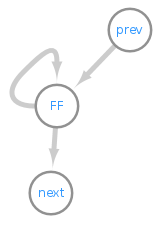
\includegraphics[scale=1.0]{figuras/dataflow/Flip_flop.png}}
    \caption{FF identifica o nó de flip flop.}
    \label{fig:flipFlop}
\end{figure}

É importante ressaltar que o nó \textit{oper0} no RVND (Figura~\ref{fig:rvndGraph}) também possui uma retroalimentação contudo não é um nó de flip flop pois não retroalimenta sua própria saída, este nó não precisa da informação de sua última execução para realizar o seu processamento, desta forma possui apenas uma porta de entrada.

\subsection{Múltiplas portas de saída}\label{subsec:multiplasSaidas}

Em modelo dataflow um nó será processado quando todas as suas dependências forem satisfeitas, contudo, ao final de seu processamento o resultado pode ser enviado como entrada para um ou mais nós.
Pode ser visto na Figura~\ref{fig:dataflowMo0} que o nó \textit{MO} está conectado a um nó com informação de entrada (nó \textit{prev}) e ligado a três nós de saída (\textit{next 0}, \textit{next 1} e \textit{next 2}).

\begin{figure}[htbp]
    \centerline{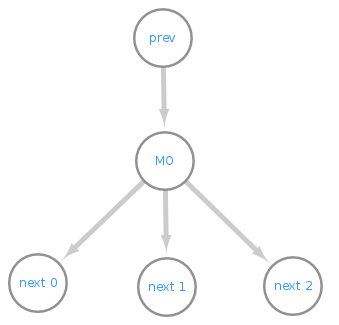
\includegraphics[scale=0.9]{figuras/dataflow/multi_output0.png}}
    \caption{Pedaço de um grafo dataflow em que o nó \textit{MO} do datalflow possui múltiplas saídas.}
    \label{fig:dataflowMo0}
\end{figure}

No modelo atual de implementação da biblioteca Sucuri é possível que um nó receba informações de vários outros nós contudo existe apenas uma porta de saída a qual podem estar conectados vários nós.

Pegando-se o exemplo da Figura~\ref{fig:dataflowMo3}, quando o nó \textit{MO} termina de processar seu resultado é enviado para a única porta de saída existente a qual estão ligados os nós \textit{next 0}, \textit{next 1} e \textit{next 2}, dessa forma todos os nós seguintes vão receber a informação e estarão aptos para processamento mesmo que a informação não seja destinada a eles.
Cada um desses nós terá então que verificar se a mensagem é destinada a ele antes de processar ou não a informação.

\begin{figure}[htbp]
    \centerline{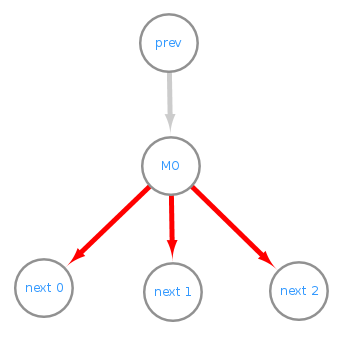
\includegraphics[scale=0.9]{figuras/dataflow/multi_output3.png}}
    \caption{Quando o nó \textit{MO} termina de processar seu resultado é enviado para todos os nós subsequentes (\textit{next 0}, \textit{next 1} e \textit{next 2}).}
    \label{fig:dataflowMo3}
\end{figure}

Foi implementada a alteração exemplificada na Figura~\ref{fig:dataflowMo1}, nesse caso existe uma porta de saída para cada nó ligado ao nó \textit{MO}, este identifica os destinatários da mensagem e aciona apenas aqueles necessários.

\begin{figure}[htbp]
    \centerline{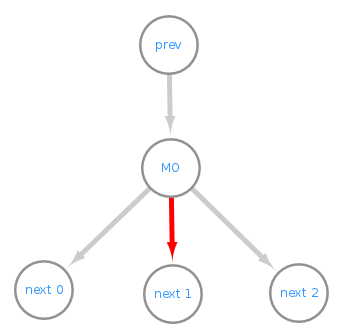
\includegraphics[scale=0.9]{figuras/dataflow/multi_output1.png}}
    \caption{Quando o nó \textit{MO} termina de processar é possível escolher qual porta de saída será utilizada e assim decidir o destino da informação.}
    \label{fig:dataflowMo1}
\end{figure}

No DVND, ao escolher o destinatário da mensagem é possível evitar uma grande quantidade de transmissões desnecessárias de mensagens, evitando assim que os nós de vizinhança sejam acionados apenas para identificar que não precisam processar a mensagem.
Vejamos, por exemplo, o nó \textit{man} da Figura~\ref{fig:dvndGraph} sem o artifício de múltiplas portas de saída todas as mensagens serão enviadas para todas as 5 vizinhanças e para o nó finalizador (\textit{end}) sendo que a mensagem só é enviada para os nós ociosos naquele momento.

A implementação de múltiplas portas de saída trás vantagens ainda mais significativas quando o tamanho da mensagem a ser transmitido é grande e quando a execução do processamento está sendo feita em um ambiente de mais de uma máquina o que envolve troca de mensagens pela rede.

\section{GDVND}\label{subsec:gdvnd}

Trazendo o conceito de \textit{movimentos independentes} (discutido na Seção \ref{subsubsec:movimentosIndependentes}) para o DVND surge a ideia do \emph{Generalized Distributed Variable Neighborhood Descent} (\emph{GDVND}).
A ideia do GDVND é um DVND que trabalha no escopo de movimentos de melhora e não em melhores soluções.
No DVND, a cada iteração o método recebe uma nova solução de uma das vizinhanças e verifica qual a melhor para então enviar esta para ser processada pelas vizinhanças ociosas que ainda não a processaram, sempre mantendo a melhor solução já encontrada.
A diferença para o GDVND é que este recebe não somente uma solução mas a solução com um conjunto de movimentos de melhora encontrado pela vizinhança, então o método tenta combinar os movimentos da melhor solução atual com aqueles da solução recebida.
Para tanto é necessário que as soluções tenham a mesma solução base, então é necessário identificar o conjunto de movimentos independentes que proporcione o maior ganho em termos de valor da solução.
Além de melhorar a solução a utilização da composição de movimentos proporciona uma melhor utilização dos recursos usados no processamento ao aproveitar computações realizadas em nós diferentes.

O grafo dataflow do GDVND é equivalente ao do DVND expresso na Figura~\ref{fig:dvndGraph} alterando apenas a informação trafegada entre os nós e a implementação interna do nó gerenciador, conforme Algoritmo~\ref{alg:gdvndMan}, ao qual caberá combinar os movimentos de vizinhanças diferentes.
Na linha \ref{alg:gdvndMan:merge} é chamado o processo combinar movimentos que pode ser visto em mais detalhes no Algoritmo~\ref{alg:gdvndMergeFunc}.
Os movimentos são combinados para formar uma solução resultante, tomando proveito do Teorema da independência de movimentos dois a dois (Teorema~\ref{teo:independenciaMovimentos2a2}) o valor da solução resultante pode ser calculado para dois movimentos, sem a necessidade de recalcular toda a solução, o que é particularmente útil para grandes instâncias e problemas cujo cálculo da função objetivo é muito caro computacionalmente.
Pode-se utilizar o mesmo teorema para estimar o valor das soluções na composição de mais de dois movimentos dois a dois.

\begin{algorithm}[htpb]
\caption{Nó \textit{man} do GDVND}
\label{alg:gdvndMan}
\begin{algorithmic}[1]
    \Function{GDVND\_Man}{Solução: $s$, Histórico: $H$, Vizinhança: $k$}
        \Let{$s_{merged}$}{$GDVND\_merge(s, bestSolution(H))$} \label{alg:gdvndMan:merge} \Comment{Combina a solução atual com a melhor conhecida}
        \Let{$H(k)$}{$min(s, s_{merged}, bestSolution(H))$} \Comment{Atualiza o histórico da vizinhança $k$ com a melhor solução}
        \Return{SoluçãoBase($H(k)$), Movimentos($H(k)$)}
    \EndFunction
\end{algorithmic}
\end{algorithm}

Seja um grafo $G = (V, E)$ cujos vértices $V$ são movimentos e as arestas $E$ indicam se um movimento é independente de outro.
Dessa forma encontrar o melhor sub-conjunto de movimentos independentes entre si dois a dois corresponderia a encontrar o sub-grafo completo correspondente ao clique maximal em que o o somatório do valor dos vértices seja máximo.

Neste trabalho é usada uma heurística para encontrar o melhor sub-conjunto de movimentos independentes, o Algoritmo~\ref{alg:gdvndMergeFunc} ilustra a heurística utilizada para fazer o \emph{merge} dos movimentos da solução.
O método apenas pode ser executado quando as soluções base são iguais para as duas soluções de entrada.
Os movimentos são reunidos num conjunto $M'$ e então ordenados conforme a melhoria que podem aplicar à solução.
Em seguida cada movimento é testado, em busca de conflitos, contra as demais movimentos, caso haja conflito este movimento é descartado, os movimentos foram dispostos de forma que os movimentos com pior resultado sobre a solução sejam testados primeiro, desta forma aqueles com melhores valores são deixados por último para que possam ser preservados caso possuam conflitos com algum outro.

\begin{algorithm}[htpb]
\caption{Combinando movimentos de soluções diferentes}
\label{alg:gdvndMergeFunc}
\begin{algorithmic}[1]
    \Function{GDVND\_merge}{Solução: $s_1$, Solução: $s_2$}
        \If{SoluçãoBase($s_1$) = SoluçãoBase($s_2$)} \Comment{Somente soluções com a mesma solução base podem ser combinadas}
            \Let{$M'$}{sorted(Movimentos($s_1$) $\cup$ Movimentos($s_2$))} \Comment{Movimentos ordenados pelo valor da melhoria na solução}
            \For{$i \gets 0$ to $len(M')$}
                \For{$j \gets (i + 1)$ to $len(M')$}
                    \If{$m_i \nparallel m_j$}
                        \Let{$M'$}{$M' - {m_i}$}
                        \State break
                    \EndIf
                \EndFor
            \EndFor
            \Return{SoluçãoBase($s_1$), $M'$}
        \EndIf
        \Return{$min(s_1, s_2)$}
    \EndFunction
\end{algorithmic}
\end{algorithm}

O retorno da iteração de cada vizinhança do GDVND passa a corresponder não a uma solução $s'$ mas a uma tupla com a solução e os movimentos aplicados, assim temos a resposta como $(s', \{m_1^x, m_2^x, \dots, m_k^x\})$.

É importante ressaltar a diferença do \emph{Multi Improvement} para o GDVND, o primeiro é uma estratégia de exploração de vizinhanças em que a busca local avança de uma solução para outra fazendo uso de uma composição de movimentos independentes $\{m_1^x, m_2^x, \dots, m_k^x\} \subset M^x$ pertencentes a uma vizinhança, no caso do GDVND os movimentos independentes são oriundos de todas as vizinhanças utilizadas pelo algoritmo.
Ainda na analogia com o \emph{Multi Improvement}, o GDVND poderia ser visto como um \emph{multi improvement} em que a sua vizinhança é a união de todas as vizinhanças utilizadas no GDVND.

A mesma ideia pode ser aplicada para um conjunto de movimentos $M = \{ m_1, m_2, m_3, ...\}$, ditos independentes se para uma solução $s$ qualquer e para todo subconjunto não-vazio $M' = \{ m_1, m_2, m_3, ..., m_k \} \subseteq M$ temos $\widehat{m_1}(s) + \widehat{m_2}(s) + \widehat{m_3}(s) + ... + \widehat{m_k}(s) = \widehat{m_1}(m_2 \circ m_3 \circ ...\circ m_k \circ s)$. 
Utilizaremos a letra $I$ para denotar movimentos independentes, por exemplo, $I(\{m_3, m_5, m_9\})$.

\subsection{Detecção movimentos independentes} \label{subsec:gdvndDetectarMovimentosIndependentes}

Para detectar quais movimentos são independentes, uma estrutura de dados $C$ para gerenciamento de conflitos foi proposta.
No caso do problema em questão, a estrutura se trata de vetor com $N$ bits, onde cada bit $i$ indica se houve alguma alteração relativa ao cliente $i$.

Exemplo $C: |0|0|0|1|1|1|1|0|0|0|0|0|0|$

Assim, a estrutura $C$ começa com todos bits zero, considerando uma solução de referência $s$.
Cada movimento altera a estrutura $C$ além de alterar a solução corrente, indicando quais posições estão comprometidas.
Da mesma maneira, uma função $d$ de detecção de conflitos indica se um movimento é "aplicável" dada certa configuração da estrutura de conflitos.

Dessa forma, ao aplicar um movimento, se for necessário alterar um bit para 1 que já tenha valor 1 então o movimento atual é conflitante com o anterior ou algum dos anteriores.

Como podemos ver a seguir a detecção de conflitos para uma solução de tamanho $n=13$, os movimentos $Swap_{1,3} \parallel Swap_{5,9}$, $Swap_{5,9} \parallel Swap_{3,7}$ mas $Swap_{1,3} \nparallel Swap_{3,7}$.\\
$C:$ |0|\textbf{0}|0|\textbf{0}|0|0|0|0|0|0|0|0|0| - $Swap_{1,3}$ \\
$C:$ |0|1|0|1|0|\textbf{0}|0|0|0|\textbf{0}|0|0|0| - $Swap_{5,9}$ \\
$C:$ |0|1|0|\textbf{1}|0|1|0|\textbf{0}|0|1|0|0|0| - $Swap_{3,7}$ \\
$C:$ |0|1|0|\textcolor{red}{0}|0|1|0|1|0|1|0|0|0| - Conflito \\
A estrutura começa com todos os bits com valor zero, os bits em negrito indicam aqueles que serão alterados pelo movimento atual, na última linha o bit em vermelho indica a existência de um conflito ($Swap_{1,3} \nparallel Swap_{3,7}$).

\subsection{Exemplo de execução} \label{subsec:gdvndExemplo}

No DVND, várias buscas começam de uma mesma solução de referência e o melhor movimento (ou primeiro de melhora) é retornado como candidato à inclusão em um pool de movimentos, chamado Histórico.
Este pool pode ser visto como um grafo não direcionado, no qual os vértices são movimentos e arestas indicam conflitos entre movimentos.
Porém, setas especiais são utilizadas para marcar dependência entre movimentos. Se $m_B$ depende de $m_A$, então $m_B$ só pode ser aplicado se $m_A$ for aplicado antes na solução.
Escolhendo o maior (ou menor) conjunto independente neste grafo, respeitando os conflitos e dependências, resultará na melhor combinação de movimentos em um dado momento, considerando múltiplas estruturas de vizinhança simultaneamente.

A Figura~\ref{fig:exemplo-dvnd} apresenta um exemplo do grafo de Histórico para uma execução do GDVND com três processos de busca.

\begin{figure}[htpb]
    \centering
    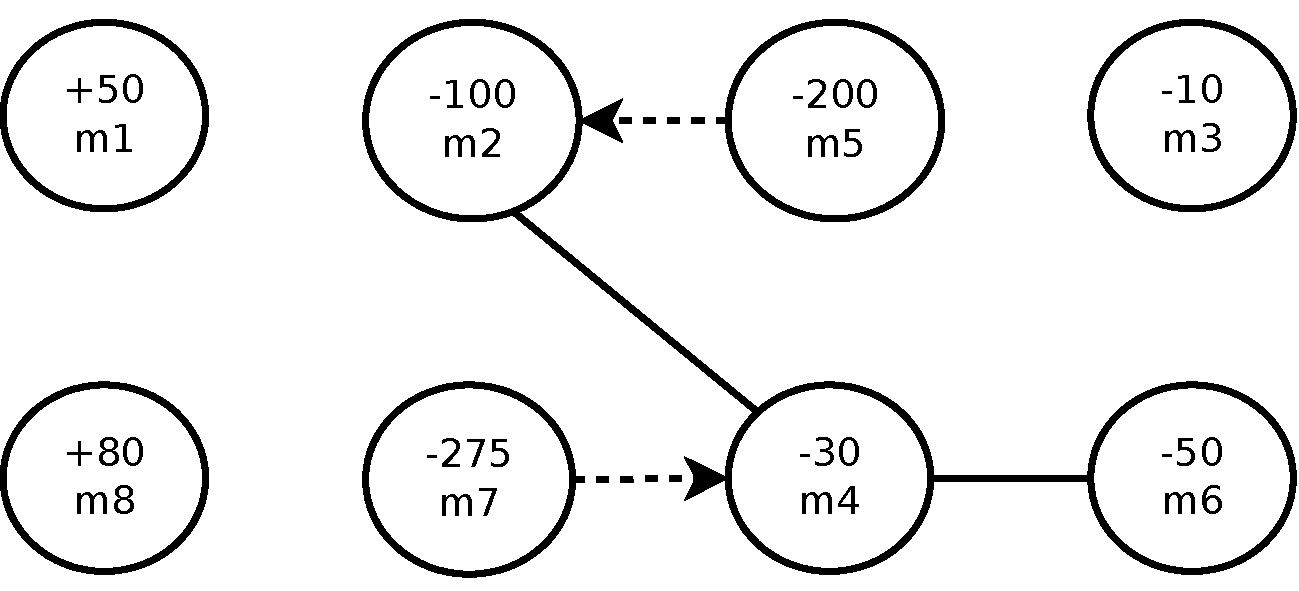
\includegraphics[width=0.65\linewidth]{figuras/gdvnd/dvnd_exemp.pdf}
    \caption{Exemplo de um grafo de Histórico.
    A combinação ótima de custos consiste nos movimentos $m_2$, $m_3$, $m_5$ e $m_6$.
    \label{fig:exemplo-dvnd}}
\end{figure}

Para entender melhor a ideia do algoritmo, a tabela abaixo simula a execução do algoritmo para três processos.

\begin{table}[htpb]
\centering
\caption{Execução do GDVND}
\begin{tabular}{|c|cccc|c|}
\hline
    \# & $f$ & solução & direção & processo & conflito\\\hline
    1  & 1000 & $s_1$ & $\rightarrow$ & P1 &\\
    2  & 1000 & $s_1$ & $\rightarrow$ & P2 &\\
    3  & 1000 & $s_1$ & $\rightarrow$ & P3 &\\\hline
    4  & 970 & $m_4 \circ s_1$ & $\leftarrow$ & P3 &\\
    5  & 970 & $m_4 \circ s_1$ & $\rightarrow$ & P3 &\\\hline
    6  & 900 & $m_2 \circ s_1$ & $\leftarrow$ & P1 & \\
    7*  & 900 & $m_2 \circ s_1$ & $\rightarrow$ & P1 & $m_2 \nparallel m_4$\\\hline
    8  & 1050 & $m_1 \circ s_1$ & $\leftarrow$ & P2 &\\
    9*  & 900 & $m_2 \circ s_1$ & $\rightarrow$ & P2 &\\\hline
    10 & 890 & $m_3 \circ m_2 \circ s_1$ & $\leftarrow$ & P1 & \\
    11 & 890 & $m_3 \circ m_2 \circ s_1$ & $\rightarrow$ & P1 & $m_2 \parallel m_3$\\\hline
    12 & 700 & $m_5 \circ m_2 \circ s_1$ & $\leftarrow$ & P2 &\\
    13 & 690 & $m_5 \circ m_3 \circ m_2 \circ s_1$ & $\rightarrow$ & P2 & $m_3 \parallel m_5$ e $m_2 \parallel m_5$\\\hline
    14 & 695 & $m_7 \circ m_4 \circ s_1$ & $\leftarrow$ & P3 &\\
    15 & 685 & $m_7 \circ m_4 \circ m_3 \circ s_1$ & $\rightarrow$ & P3 & $m_2 \nparallel m_7$ e $m_5 \nparallel m_4$\\\hline
    16 & 840 & $m_6 \circ m_3 \circ m_2 \circ s_1$ & $\leftarrow$ & P1 &\\
    17 & 640 & $m_6 \circ m_3 \circ m_5 \circ m_2 \circ s_1$ & $\rightarrow$ & P1 & $m_6 \parallel m_2, m_3, m_5$\\\hline
    18 & 765 & $m_8 \circ m_7 \circ m_4 \circ m_3 \circ s_1$ & $\leftarrow$ & P3 &\\
    19 & 640 & $m_6 \circ m_3 \circ m_5 \circ m_2 \circ s_1$ & $\rightarrow$ & P3 & $m_8 \nparallel m_6$\\\hline
\end{tabular}
\end{table}

O Histórico começa distribuindo a solução $s_1$ para cada busca, e eventualmente coleta um novo movimento e distribui uma nova solução.
Todos os cálculos são feitos sobre uma mesma solução de referência $s_1$, que só é modificada no passo 20 do algoritmo.
Nas iterações 7 e 9, note que existem conflitos a serem resolvidos (vide grafo na Figura~\ref{fig:exemplo-dvnd}).
Após a iteração 19, o Histórico percebe que os três processos tem movimentos em comum: $m_3$, $m_5$ e $m_2$. Então uma nova solução $s_2$ é armazenada no Histórico como solução de referência, sendo ela $s_2 = m_3 \circ m_5 \circ m_2 \circ s_1$ (de custo 690).
Assim, os processos P1 e P3 continuam naturalmente processando a solução $m_6 \circ s_2$ (antiga $m_6 \circ m_3 \circ m_5 \circ m_2 \circ s_1$), e P2 continua com $s_2$ (antiga $m_5 \circ m_3 \circ m_2 \circ s_1$).
Note também que, ao adotar estes três movimentos, todos movimentos com conflitos (ou dependência de algum movimento em conflito) tem de ser eliminados. Então, $m_4$ e $m_7$ são descartados.
Vale observar que $m_1$ e $m_8$ nunca foram armazenados, pois eram de piora.
O grafo final então consiste somente dos movimentos $m_6$, $m_3$, $m_5$ e $m_2$.

%OBSERVAÇÃO IMPORTANTE: eu acho que este processo pode ser mais estável se a unificação ocorrer após UMA iteração que o conjunto de movimentos comuns se mantenha estável, mas teremos que experimentar para saber =D

\begin{table}[htpb]
\centering
\caption{Consolidação de uma nova solução no GDVND}
\begin{tabular}{|c|ccc|}
\hline
\# & $f$ & solução & local\\\hline
20 & 690 & $s_2 = m_3 \circ m_5 \circ m_2 \circ s_1$ &  Histórico\\
   & 640 & $m_6 \circ s_2$ & P1\\
   & 690 & $s_2$           & P2\\
   & 640 & $m_6 \circ s_2$ & P3\\\hline
\end{tabular}
\end{table}

\subsection{Controle de execução entre CPU e GPU}

Para entender como o método tira proveito da arquitetura híbrida CPU-GPU segue o presente exemplo:
A CPU é utilizada para decidir qual solução cada processo de busca local irá utilizar, minimizando as transferências de memória CPU-GPU. % e, assim, maximizando o aproveitamento na estrutura de dados ADS (informações auxiliares usada para acelerar o cálculo do valor da solução) das na memória da GPU.

EXEMPLO:\\
 Processo A $\rightarrow$ CPU\\
 Processo B $\rightarrow$ Kernel GPU Swap\\
 Processo C $\rightarrow$ Kernel GPU 2-Opt\\
 Processo D $\rightarrow$ Kernel GPU Or-1\\
 Processo E $\rightarrow$ Kernel GPU Or-2\\
 Processo F $\rightarrow$ Kernel GPU Or-3

Solução $s_1$ = [1,2,3,4,5,6,7,8,9,10], ($f(s_1) = 1000$).

A solução $s_1$ entra na GPU para todas as buscas B-F, cada uma em um fluxo (\emph{thread}) distinto.
Supomos que o processo B (Swap) termina antes com ganho -100 (melhora, $\widehat{m_1} = -100$) na troca $m_1 = Swap_{2,5}$.
A CPU então cria $s_2 = m_1 \circ s_1$.
Como $s_2$ é a melhor solução atual, ela é copiada para a GPU, e o processo B roda em cima de $s_2$ = [1,5,3,4,2,6,7,8,9,10], com $f(s_2) = 900$.

Neste momento, o processo D termina com $m_2 = Or-1_{7,9}$, movendo cliente 7 para depois do 9, com ganho -50, $\widehat{m_2} = -50$.
A CPU então analisa $m_1$ e $m_2$, como não há conflitos uma solução $s_3 = m_2 \circ m_1 s_1$ é criada para o processo D executar. $s_3$=[1,5,3,4,2,6,8,9,7,10], com $f(s_3) = 850$

O processo C termina com o movimento $m_3=2Opt_{1,3}$ (inverte de 1 a 3) com ganho -120 ($\widehat{m_3} = -120$.
A CPU percebe que $m_3 \nparallel m_1$, mas $m_3 \parallel m_2$.
Então a solução $s_4= m_4 \circ m_2 \circ s_1$ é gerada e passada à GPU para o processo C, com $f(s_4) = 830$

O processo E termina sem ganho com o movimento $m_4 = Or-2_{1,4}$ (move clientes 1,2 para depois do 4).
A CPU percebe que $m_4 \nparallel m_1$ e $m_4 \nparallel m_3$ mas $m_4 \parallel m_2$.
Porém, a melhor configuração atual é $s_4$ ($f(s_4)=830$), então a busca parte dela (e ela já está na memória da GPU).

Finalmente, o processo B (Swap) termina novamente com melhora -60 e troca $m_5=Swap_{3,8}$.
Esta troca roda em cima de $s_2$, então não existem outros movimentos para haver conflito.
A solução $s_5 = m_5 \circ s_2$ com $f(s_5) = 840$ é criada, porém, a solução $s_4$ ($f(s_4) = 830$) é melhor.
A CPU então relança o processo B com a solução $s_4$.

\subsection{Passo iterativo}

Utilizando o termo convencionado na seção~\ref{subsec:passoIterativo}, cada passo iterativo do GDVND retorna a melhor solução encontrada para todas as vizinhanças combinado com a melhor solução já encontrada.
Dessa forma, sendo $N$ a união de todas as vizinhanças, contudo a resposta do GDVND pode conter mais de um movimento combinados simultaneamente, assim convencionaremos chamar de $\mathcal{N} = \{ m_1 \circ m_2 \circ \dots \circ m_z \circ s \mid \forall m_i \in \mathcal{M} \land \forall i, j \quad m_i \parallel m_j \}$, podemos ver, pela definição de $\mathcal{N}$, que $N \subset \mathcal{N}$ pois qualquer elemento de $N$ pode ser escrito da forma $m_1 \circ s$ que também pertence a $\mathcal{N}$.
Assim o passo iterativo do GDVND pode ser dado pela Equação~\ref{eq:gdvndPassoIterativo}.

\begin{equation} \label{eq:gdvndPassoIterativo}
\rho^{GDVND}(s) = s' \in \mathcal{N} \  \textrm{sendo} \  f(s') < f(s''), \forall s'' \in \mathcal{N}(s) \  \textrm{com} \  s'' \ne s
\end{equation}

Fazendo uso da notação de movimentos podemos escrever \ref{eq:dvndPassoIterativo} como a Equação~\ref{eq:dvndPassoIterativoMovimento}.

\begin{equation} \label{eq:gdvndPassoIterativoMovimento}
\rho^{GDVND}(s) = m_1 \circ m_2 \circ \dots \circ m_z \circ s \  \textrm{sendo} \  m \in \mathcal{M} \land \forall i,j \quad m_i \parallel m_j \  \textrm{com} \  i \ne j
\end{equation}

Pelo passo iterativo do RVND $\rho^{RVND}$ (\ref{eq:rvndPassoIterativoMovimento}), do DVND $\rho^{DVND}$ (\ref{eq:dvndPassoIterativoMovimento}) e do GDVND $\rho^{GDVND}$ (\ref{eq:gdvndPassoIterativoMovimento}) podemos concluir que $\rho^{GDVND}(s) \le \rho^{DVND}(s) \le \rho^{RVND}(s)$, contudo novamente isso não é suficiente para afirmar que o GDVND encontre necessariamente melhores resultados pois o pode acabar convergindo muito cedo para um mínimo local.

À primeira vista pode parecer que pela vizinhança do passo iterativo do GDVND conter as vizinhanças do RVND e DVND contudo podemos ver que toda solução encontrada pelo GDVND pode ser gerada por um conjunto de operações do DVND ou RVND.

Para que uma solução produzida pelo GDVND não possa ser produzida pelo RVND ou DVND deve haver um movimento nessa solução que não seja possível encontrar com RVND ou DVND, suponhamos então que o GDVND produziu uma solução $m_1 \circ m_2 \circ \dots \circ m_z \circ s \in \mathcal{N}$ com $m_i \in \{ m_1, m_2, \dots, m_z \}$ tal que $m_i \notin \mathcal{M}$.
\begin{proof}
\begin{align*}
\rho^{GDVND}(s) =& m_1 \circ m_2 \circ \dots \circ m_i \circ \dots \circ m_z \circ s & \textrm{Por comutatividade} \\
\rho^{GDVND}(s) =& m_i \circ m_1 \circ m_2 \circ \dots \circ m_z \circ s & \textrm{Fazendo } s' = m_1 \circ m_2 \circ \dots \circ m_z \circ s \\
\rho^{GDVND}(s) =& m_i \circ s' & \textrm{Logo uma contradição } \bot \\
\end{align*}
\end{proof}
Quando se escreve $\rho^{GDVND}(s) = m_i \circ s'$ chega-se a uma contradição pois, pela definição do passo iterativo do GDVND, temos que o movimento $m_i$ deveria pertencer ao conjunto $\mathcal{M}$ contudo supôs-se por hipótese que $m_i \notin \mathcal{M}$.

\section{Vizinhanças}\label{sec:neighborhoods}

% Vizinhanças Swap, 2-opt, 1-OrOpt, 2-OrOpt, 3-OrOpt
RVND, DVND e GDVND usam um conjunto de vizinhanças para processar a solução, foram escolhidas 5 estruturas diferentes, a saber, Swap, 2-Opt, OrOpt-1, OrOpt-2 e OrOpt-3, as mesmas utilizadas em~\cite{wamca2016}.
% Nesse caso o DVND pode, potencialmente, demandar 5 vezes o tempo computacional necessário pelo RVND no pior cenário (quando a exploração do RVND é ótima) pois no RVND cada solução é propagada para apenas uma vizinhança quando não é encontrada uma melhora.
No caso do DVND, a cada nova solução encontrada esta pode ser submetida para todas as vizinhanças simultaneamente (tentando explorar melhorias de vizinhanças diferentes simultaneamente).
% O desafio para melhorar o DVND frente ao RVND é explorar as vizinhanças e combinar os movimentos, de modo a evitar a geração desnecessária de soluções que causariam um desperdício de recursos computacionais.
% This idea will still be expanded in future works, as for now we lack the capability to combine moves from different neighborhoods, so it is expected to have DVND consuming bigger computational times than RVND.
A intenção principal é prover uma implementação dataflow de um procedimento de busca local de muitas vizinhanças, o que é uma contribuição original para ambas comunidades, de otimização e computação paralela.

Para a busca local foi usado uma abordagem \emph{Multi Improvement} (\emph{MI})~\cite{wamca2016} em todas as vizinhanças, na qual é calculado os custos de todos os movimentos e os resultados armazenados num vetor.
Usando a estratégia \emph{Best Improvement} (\emph{BI}) apenas a melhor solução é selecionada, na estratégia \emph{Multi Improvement} todos os \textit{movimentos independentes} são simultaneamente aplicados para a solução dada, provendo assim uma convergência mais rápida para o ótimo local.

A enumeração de todos as estratégias de vizinhança roda numa implementação em GPU, assim temos um algoritmo dataflow onde a implementação de cada nó \textit{oper} roda em GPU para ambos os casos, a configuração do lançamento do \emph{kernel} para cada estratégia de vizinhança é descrita na Tabela~\ref{tab:neighborhoodsLaunchConfigurarion}, estas configurações foram obtidas fazendo-se uso das bibliotecas fornecidas pela NVIDIA para otimização do uso dos recursos conforme o \emph{kernel} que se deseja executar, conforme descrito em~\cite{cudaProTipOccupancy}
Mais detalhes sobre a implementação GPU da enumeração das vizinhanças podem ser encontrados em \cite{wamca2016}.

% Aqui eu coloquei essa informação porque o revisor pediu, mas devo colcocar como obtenho cada configuração?

\begin{table}[ht]
\centering
\caption{Configuração de lançamento para os kernels das vizinhanças.
Onde \textit{Grid} refere-se a quantidade de grides usada, \textit{Block} o tamanho de cada bloco de threads e \textit{Shared} indica a quantidade de memória compartilhada utilizada pelas threads em cada bloco.}
\label{tab:neighborhoodsLaunchConfigurarion}
\begin{tabular}{llllllll}
\hline
\hline
\textbf{Instância} & \textbf{n} & \textbf{Vizinhança} & \textbf{Grid} & \textbf{Block} & \textbf{Shared} \\ \hline
\multirow{5}{*}{\#0 \rotatebox[origin=c]{90}{berlin52}} & \multirow{5}{*}{52} & Swap         & 26      & 53      & 1060   \\
                            & &  2-Opt        & 27      & 53      & 1060   \\
                            & & OrOpt-1      & 50      & 53      & 1060   \\
                            & & OrOpt-2      & 49      & 53      & 1060   \\ 
                            & & OrOpt-3      & 48      & 53      & 1060   \\ \hline
\multirow{5}{*}{\#1 \rotatebox[origin=c]{90}{kroD100}} & \multirow{5}{*}{100} & Swap         & 50      & 101      & 2020   \\
                            & & 2-Opt        & 51      & 101      & 2020   \\
                            & & OrOpt-1      & 98      & 101      & 2020   \\
                            & & OrOpt-2      & 97      & 101      & 2020   \\ 
                            & & OrOpt-3      & 96      & 101      & 2020   \\ \hline
\multirow{5}{*}{\#2 \rotatebox[origin=c]{90}{pr226}} & \multirow{5}{*}{226} & Swap         & 113      & 224      & 4540   \\
                            & & 2-Opt        & 114      & 224      & 4540   \\
                            & & OrOpt-1      & 224      & 224      & 4540   \\
                            & & OrOpt-2      & 223      & 224      & 4540   \\ 
                            & & OrOpt-3      & 222      & 224      & 4540   \\ \hline
\multirow{5}{*}{\#3 \rotatebox[origin=c]{90}{lin318}} & \multirow{5}{*}{318} & Swap         & 159      & 256      & 6380   \\
                            & & 2-Opt        & 160      & 256      & 6380   \\
                            & & OrOpt-1      & 316      & 256      & 6380   \\
                            & & OrOpt-2      & 315      & 256      & 6380   \\ 
                            & & OrOpt-3      & 314      & 256      & 6380   \\ \hline
\multirow{5}{*}{\#4 \rotatebox[origin=c]{90}{TRP-S500-R1}} & \multirow{5}{*}{501} & Swap         & 250      & 502      & 10040   \\
                            & & 2-Opt        & 251      & 502      & 10040   \\
                            & & OrOpt-1      & 499      & 502      & 10040   \\
                            & & OrOpt-2      & 498      & 502      & 10040   \\ 
                            & & OrOpt-3      & 497      & 502      & 10040   \\ \hline
\multirow{5}{*}{\#5 \rotatebox[origin=c]{90}{d657}} & \multirow{5}{*}{657} & Swap         & 328      & 512      & 13160   \\
                            & & 2-Opt        & 329      & 512      & 13160   \\
                            & & OrOpt-1      & 655      & 512      & 13160   \\
                            & & OrOpt-2      & 654      & 512      & 13160   \\ 
                            & & OrOpt-3      & 653      & 512      & 13160   \\ \hline
\multirow{5}{*}{\#6 \rotatebox[origin=c]{90}{rat784}} & \multirow{5}{*}{783} & Swap         & 391      & 672      & 15680   \\
                            & & 2-Opt        & 392      & 672      & 15680   \\
                            & & OrOpt-1      & 781      & 672      & 15680   \\
                            & & OrOpt-2      & 780      & 672      & 15680   \\ 
                            & & OrOpt-3      & 779      & 672      & 15680   \\ \hline
\multirow{6}{*}{\#7 \rotatebox[origin=c]{90}{TRP-S1000-R1}} & \multirow{5}{*}{1001} & Swap         & 500      & 1002      & 20040   \\
                            & & 2-Opt        & 501      & 1002      & 20040   \\
                            & & OrOpt-1      & 999      & 1002      & 20040   \\
                            & & OrOpt-2      & 998      & 1002      & 20040   \\ 
                            & & OrOpt-3      & 997      & 1002      & 20040   \\
                            & &              &          &           &    \\
\hline
\end{tabular}
\end{table}

\subsection{Tabela de conflitos}

Para classificação de movimentos independentes é necessário identificar quando um movimento aplicado a uma solução não conflita com outro movimento aplicado a mesma solução, conforme a definição estabelecida na Seção~\ref{subsubsec:movimentosIndependentes}.

A identificação de conflitos pode ser feita em $\mathcal{O}(n)$ conforme descrito na Seção~\ref{subsec:gdvndDetectarMovimentosIndependentes}, contudo nos termos deste trabalho que trata do Problema da Mínima Latência (conforme descrito na Seção~\ref{sec:mlp}), para as vizinhanças \textit{swap}, \textit{2-opt} e \textit{oropt-k} utilizadas, dois movimentos são independentes quando são satisfeitas as condições expressas na Tabela~\ref{tab_confict}, desta forma é possível identificar a a independência de movimentos em $\mathcal{O}(1)$ independente da solução base considerada.

\begin{table}[htpb]
    \small
    \centering
    \begin{tabular}{c|c|c|c}
                          & $\mbf{swap(i_2,j_2)}$             & $\mbf{2-opt(i_2,j_2)}$    & $\mbf{oropt-k_2(i_2,j_2)}$ \\
        \hline
        %\multirow{4}{*}{\mbf$swap(i_1,j_1)$}    
                          & $(|i_1-i_2| > 1) \land$         & $[(i_1 < i_2-1) \lor$     & $(j_1 < \min(i_2,j_2)-1)\,\,\, \lor  $ \\
		$\mbf{swap}$        & $(|i_1-j_2| > 1) \land$  		& $ (i_1 > j_2-1)] \land$   & $(i_1 > \max(i_2,j_2)+k_2) \lor  $ \\
		$\mbf{(i_1,j_1)}$   & $(|j_1-i_2| > 1) \land$  		& $[(j_1 < i_2-1) \lor$     & $[(i_1 < \min(i_2,j_2)-1)\,\,\, \land $ \\
			              & $(|j_1-j_2| > 1) \,\,\,$ 		& $ (j_1 > j_2+1)]\,\,\,\,$ & $\,\,\,(j_1 > \max(i_2,j_2)+k_2)] \,\,\,$ \\
        \hline 
        %\multirow{4}{*}{\mbf$2$-$opt(i_1,j_1)$} 
                          & $[(i_2 < i_1-1) \lor$    		& $(j_1 < i_2 - 1) \lor$   & \\
		$\mbf{2-opt}$	  & $ (i_2 > j_1+1)] \land$  		& $(i_1 > j_2 + 1) \lor$   & $(i_1 > \max(i_2,j_2)+k_2) \lor$   \\
		$\mbf{(i_1,j_1)}$	  & $[(j_2 < i_1-1)] \lor$   		& $(j_2 > i_1 - 1) \lor$   & $(j_1 < \min(i_2,j_2)-1) \,\,\,\,$ \\
			              & $ (j_2 > j_1+1)]\,\,\,$  		& $(i_2 > j_1 + 1)\,\,\,$  & \\
        \hline
        %\multirow{4}{*}{\mbf$oropt$-$k_1(i_1,j_1)$} 
                          & $(j_2  < \min(i_1,i_2)-1)\,\,\, \lor$	    &   				                & \\
		$\mbf{oropt-k_1}$ & $(i_2  > \max(i_1,i_2)+k_1) \lor$           & $(j_2 < \min(i_1,j_1)-1) \lor$ & $[\max(i_1,j_1)+k_1 < \min(i_2,j_2)] \lor$ \\
		$\mbf{(i_1,j_1)}$	  & $[(i_2 < \min(i_1,i_2)-1)\,\,\land$   	    & $(i_2 > \max(i_1,j_1)+k_1)$  & $[\min(i_1,j_1) > \max(i_2,j_2)+k_2]\,\,\,\,$\\
			              & $\,\,\,\,(j_2  > \max(i_1,i_2)+k_1)]\,\,\,$ &    	                            &  \\
    \end{tabular}
    \caption{Tabela de movimentos independentes (não conflitantes)}
    \label{tab_confict}
\end{table}

\section{Decomposição de vizinhanças (Disaggregated Neighborhoods)} \label{subsec:metodologiaDecomposicaoVizinhancas}

Pela Figura~\ref{fig:dvndGraph} podemos perceber que o paralelismo horizontal, isto é, aquele obtido pela utilização de mais máquinas, neste método está limitado a quantidade de vizinhanças utilizadas no método DVND.
Esta limitação representa um problema pois para obter melhor utilização do paralelismo horizontal seria necessário também adicionar novas estruturas de vizinhanças, o que aumentaria o esforço computacional e não necessariamente traria ganho de performance ou na qualidade do valor da solução.

Contudo este problema pode ser facilmente solucionado pela decomposição das vizinhanças, isto é, no lugar de um nó \textit{oper} representar toda uma estrutura de vizinhança, este passa a processar uma sub-parte desta.
% Por exemplo, na Figura~\ref{fig:operadorSwap} temos uma vizinhança de tamanho $\mathcal{O}(n^2)$ em que cada elemento é trocado com todos os elementos subsequentes, conforme pode ser visto na Figura~\ref{fig:vizinhancaTrocas} cada elemento tem um grupo independente de trocas.

\begin{figure}[htbp]
    \centerline{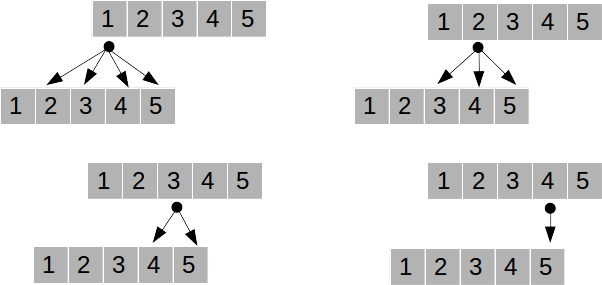
\includegraphics[scale=0.6]{figuras/vizinhanca.png}}
    \caption{Vizinhança com suas trocas para $n=5$.}
    \label{fig:vizinhancaTrocas}
\end{figure}

Isto posto, podemos separar a vizinhança em sub-grupos, um exemplo poderia ser a Figura~\ref{fig:vizinhancaTrocasDividida} que mostra a mesma vizinhança da Figura~\ref{fig:vizinhancaTrocas} dividida em dois sub-grupos. Desta forma cada sub-grupo representaria um nó \textit{oper} do diagrama dataflow DVND aumentando assim a escalabilidade horizontal do método.

\begin{figure}[htbp]
    \centerline{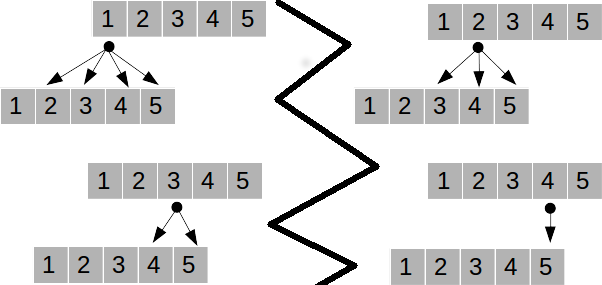
\includegraphics[scale=0.6]{figuras/vizinhancaDividida.png}}
    \caption{Vizinhança com suas trocas dividida para $n=5$.}
    \label{fig:vizinhancaTrocasDividida}
\end{figure}

A vizinhança na Figura~\ref{fig:vizinhancaTrocasDividida} exemplifica a sub-divisão em dois grupos de vizinhança contudo esta divisão limita-se apenas ao tamanho da solução proporcionando um grande potencial para o desenvolvimento do paralelismo horizontal de qualquer vizinhança sem aumentar demasiadamente o custo computacional do método.
